\documentclass[12pt]{article}
\usepackage[left=1cm, right=1cm, top=2cm,bottom=1.5cm]{geometry} 

\usepackage[parfill]{parskip}
\usepackage[utf8]{inputenc}
\usepackage[T2A]{fontenc}
\usepackage[russian]{babel}
\usepackage{enumitem}
\usepackage[normalem]{ulem}
\usepackage{amsfonts, amsmath, amsthm, amssymb, mathtools}

\usepackage{fancyhdr}
\pagestyle{fancy}
\renewcommand{\headrulewidth}{1.5pt}
\renewcommand{\footrulewidth}{1pt}

\usepackage{graphicx}
\usepackage[figurename=Рис.]{caption}
\usepackage{subcaption}
\usepackage{float}

%%Наименование папки откуда забирать изображения
\graphicspath{ {./images/} }

%%Изменение формата для ввода доказательства
\renewcommand{\proofname}{$\square$  \nopunct}
\renewcommand\qedsymbol{$\blacksquare$}

\addto\captionsrussian{%
	\renewcommand{\proofname}{$\square$ \nopunct}%
}
%% Римские цифры
\newcommand{\RN}[1]{%
	\textup{\uppercase\expandafter{\romannumeral#1}}%
}

%% Для удобства записи
\newcommand{\MR}{\mathbb{R}}
\newcommand{\MQ}{\mathbb{Q}}
\newcommand{\MI}{\mathrm{I}}
\newcommand{\MJ}{\mathrm{J}}
\newcommand{\MU}{\mathcal{U}}
\newcommand{\VN}{\varnothing}
\newcommand{\VE}{\varepsilon}

\theoremstyle{definition}
\newtheorem{defn}{Опр:}
\newtheorem{rem}{Rm:}
\newtheorem{prop}{Утв.}
\newtheorem{exrc}{Упр.}
\newtheorem{lemma}{Лемма}
\newtheorem{theorem}{Теорема}
\newtheorem{corollary}{Следствие}

\newenvironment{cusdefn}[1]
{\renewcommand\thedefn{#1}\defn}
{\enddefn}

\DeclareRobustCommand{\divby}{%
	\mathrel{\text{\vbox{\baselineskip.65ex\lineskiplimit0pt\hbox{.}\hbox{.}\hbox{.}}}}%
}
\DeclareMathSymbol{\SMN}{\mathbin}{AMSa}{"39}

\newcommand{\smallerrel}[1]{\mathrel{\mathpalette\smallerrelaux{#1}}}
\newcommand{\smallerrelaux}[2]{\raisebox{.1ex}{\scalebox{.75}{$#1#2$}}}

\newcommand{\smallin}{\smallerrel{\in}}
\newcommand{\smallnotin}{\smallerrel{\notin}}

\newcommand*{\medcap}{\mathbin{\scalebox{1.25}{\ensuremath{\cap}}}}%
\newcommand*{\medcup}{\mathbin{\scalebox{1.25}{\ensuremath{\cup}}}}%

\begin{document}
	\lhead{Математический анализ - I}
	\chead{Шапошников С.В.}
	\rhead{Лекция - 21}

\section*{Сходимость функций}
\begin{defn}
	$f_n \to f$ \uwave{поточечно на множестве $D$}, если $\forall x \in D, \, f_n(x) \to f(x)$.
\end{defn}

При поточечной сходимости теряется свойство непрерывности. Но точек разрыва не может быть слишком много.

\begin{theorem}
	Если $f_n$ - непрерывны на $\MR \wedge \forall x\in \MR, \, f_n(x) \to f(x)$, то у функции $f$ есть хотя бы одна точка непрерывности.
\end{theorem}

\uline{\textbf{Идея}}: Будем доказывать от противного, что точек непрерывности вообще нет. Тогда найдется промежуток на котором функция будет вести себя, как функция Дирихле (то есть в каждой точке имеет положительный скачок). С другой стороны, на этом же промежутке можно найти интервал, где $f_n$ достаточно близко подойдут к функции $f$, но $f_n$ - непрерывные функции, а $f$ имеет множественные скачки $\Rightarrow$ получим противоречие.

\begin{proof}
	Предположим противное, что точки разрыва это вся числовая ось.
	
	$1)$ Тогда $\MR = \bigcup\limits_{k=1}^{\infty}\underbrace{\{\,x \colon \omega(f,x) \geq \tfrac{1}{k} \,\}}_{\text{замкнутые}}$. По теореме Бэра $\exists \, k \wedge (\alpha, \beta) \colon (\alpha, \beta)\subset \{\,x \colon \omega(f,x) \geq \tfrac{1}{k} \,\}$. \\
	Уменьшая интервал, считаем, что $\alpha < \beta$ и $[\alpha,\beta] \subset \{\,x \colon \omega(f,x) \geq \tfrac{1}{k} \,\}$.
	
	$2)$ Пусть $\VE > 0 \Rightarrow$ в каждой точке $x, \exists \, N_x \colon \forall n,m > N_x, \, |f_n(x) - f_m(x)|\leq \VE$, так как $f_n(x)$ в каждой точке $x$ сходится и выполняется условие Коши $\forall x \Rightarrow$
	$$\Rightarrow [\alpha,\beta] = \bigcup\limits_{N}\bigcap\limits_{n,m > N}\Big\{x \in [\alpha, \beta]\colon |f_n(x) - f_m(x)| \leq \VE\Big\}$$
	Множество $\{x \in [\alpha, \beta]\colon |f_n(x) - f_m(x)| \leq \VE\}$ - замкнуто ($n$ и $m$ - фиксированы). Действительно, пусть $x_k \in \{x \in [\alpha, \beta]\colon |f_n(x) - f_m(x)| \leq \VE\} \wedge x_k \to x_0 \Rightarrow |f_n(x_k) - f_m(x_k)| \leq \VE$, так как функции $f_n(x), f_m(x)$ - непрерывные, то $f_n(x_k) \to f_n(x_0) \wedge f_m(x_k) \to f_m(x_0) \Rightarrow |f_n(x_k) - f_m(x_k)| \to |f_n(x_0) - f_m(x_0)| \leq \VE \Rightarrow$\\
	$\Rightarrow x_0 \in \{x \in [\alpha, \beta]\colon |f_n(x) - f_m(x)| \leq \VE\} \Rightarrow$ множество замкнутое. \\
	Таким образом $\bigcap\limits_{n,m > N}\{x \in [\alpha, \beta]\colon |f_n(x) - f_m(x)| \leq \VE\}$ - замкнутое множество, как пересечение замкнутых множеств (любое пересечение замкнутых множеств - замкнутое).
	
	$3)$ По теореме Бэра $\exists \, N \wedge (\alpha_1,\beta_1) \subset \bigcap\limits_{n,m > N}\{x \in [\alpha, \beta]\colon |f_n(x) - f_m(x)| \leq \VE\}$. На интервале $(\alpha_1, \beta_1)$ выполняются следующие свойства:
	\begin{enumerate}[label={(\arabic*)}]
		\item $\forall x \in (\alpha_1,\beta_1), \, \omega(f,x) \geq \frac{1}{k}$;
		\item $\forall x \in (\alpha_1,\beta_1), \, \forall n,m > N, \, |f_n(x) - f_m(x)| \leq \VE$;
	\end{enumerate}
	Фиксируем $n > N$, устремляем $m$ в бесконечность $m \to \infty \Rightarrow |f_n(x) - f(x)| \leq \VE$. 
	
	$4)$ Возьмем $\VE = \frac{1}{10k}$, тогда используя неравенство треугольника получим $\forall x,y \in (\alpha_1,\beta_1)$
	$$|f_n(x) - f_n(y)| \geq |f(x) - f(y)| - |f_n(x) - f(x)| - |f_n(y) - f(y)| \geq |f(x) - f(y)| - \tfrac{1}{5k}$$ 
	Пусть $x_0 \in (\alpha_1, \beta_1)$, возьмем $\delta > 0 \colon \MU_\delta(x_0) \subset (\alpha_1,\beta_1)$. Тогда $\forall x,y \in \MU_\delta(x_0) \Rightarrow$ $$\Rightarrow \omega(f_n,\MU_\delta(x_0)) = \sup\limits_{x,y \in \MU_\delta(x_0)}|f_n(x) - f_n(y)| \geq |f_n(x) - f_n(y)| \geq|f(x) - f(y)| - \tfrac{1}{5k} \Rightarrow$$ 
	$$\Rightarrow \omega(f_n,\MU_\delta(x_0)) \geq \sup\limits_{x,y \in \MU_\delta(x_0)}|f(x) - f(y)| - \tfrac{1}{5k} = \omega(f,\MU_\delta(x_0)) - \tfrac{1}{5k}\Rightarrow$$
	Устремим $\delta \to 0 \Rightarrow$ так как $f_n$ - непрерывная, то  $\omega(f_n,\MU_\delta(x_0)) \to 0, \, \omega(f,\MU_\delta(x_0)) \to \omega(f,x_0) \Rightarrow$  
	$$\Rightarrow 0 \geq \omega(f,x_0) - \tfrac{1}{5k} \geq \tfrac{1}{k} - \tfrac{1}{5k} > 0 \Rightarrow$$ 
	$\Rightarrow$ получили противоречие.
\end{proof}

\begin{corollary}
	Множество точек непрерывности $f$ - всюду плотно, то есть во всяком интервале есть точка непрерывности.
\end{corollary}
\uline{\textbf{Идея}}: Превратить интервал в прямую, так чтобы свойства непрерывности и поточечной сходимости не исчезло.
\begin{proof}
	Пусть есть интервал $(\alpha, \beta)$, на нем есть функции $f_n(x)$ и $f(x)$. Пусть мы построили непрерывные отображения $g \colon \MR \to (\alpha, \beta) \wedge g^{-1}\colon (\alpha, \beta) \to \MR $. \\
	К примеру, $g(x) = \tan(x) \colon (\SMN\frac{\pi}{2}, \frac{\pi}{2}) \to \MR \wedge g^{-1}(x) = \arctan(x) \colon \MR \to (\SMN\frac{\pi}{2}, \frac{\pi}{2})$
	\begin{figure}[H]
		\centering
		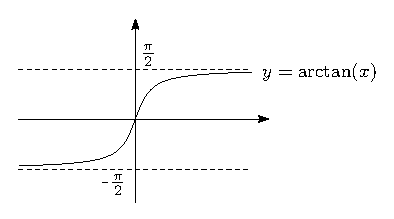
\includegraphics[width=0.4\textwidth]{21_1.eps}
		\caption{$y = \arctan(x)$.}
		\label{21_1}
	\end{figure}
	Любой интервал можно превратить в $(\SMN\frac{\pi}{2}, \frac{\pi}{2})$ линейным отображением. Составим новые функции $\tilde{f_n}(y) = f_n(g(y)) \wedge \tilde{f}(y) = f(g(y))$ - непрерывные, как композиции непрерывных функций. Поточечная сходимость есть, так как зафиксировав $y$ фиксируется и $g(y) \Rightarrow f_n(g(y)) \to f(g(y)) \Rightarrow \exists \, y_0 \in \MR \colon f(g(y))$ - непрерывна в точке $y_0$ по теореме выше.
	
	Возьмем $x_0 = g(y_0), \, f(x) = f(g(g^{-1}(x))) \Rightarrow f(g(y))$ - непрерывна в точке $y_0$, а $g^{-1}(x)$ - непрерывна в точке $x_0 \Rightarrow$ композиция непрерывных функций - непрерывна $\Rightarrow f$ - непрерывна в точке $x_0$.
\end{proof}
\begin{rem}
	Не любую функцию можно получить, как поточечный предел непрервных фнукций (например, нельзя получит функцию Дирихле).
\end{rem}

\begin{theorem}
	Пусть $f_n \colon D \to \MR, \, f \colon D \to \MR, \, a\in D$ - точка непрерывности $f_n, \, \forall n$ и $f_n$ сходятся к $f$ равномерно на $D$. Тогда $f$ непрерывна в точке $a$.
\end{theorem}

\begin{proof}
	По неравенству треугольника $|f(x) - f(a)| \leq |f(x) - f_n(x)| + |f_n(x) - f_n(a)| + |f_n(a) - f(a)|$. 
	
	$\forall \VE > 0, \, \exists \, N \colon \forall n > N, \, \forall x \in D, \, |f_n(x) - f(x)| < \VE$ - из-за равномерной сходимости. Фиксируем $n > N$, так как $f_n$ - непрерывна в точке $a$, то $\exists \, \delta>0 \colon \forall x \in D, \, |x-a| < \delta \Rightarrow |f_n(x) - f_n(a)| < \VE \Rightarrow |f(x) - f(a)| < 3\VE$.
\end{proof}

\newpage

\section*{Дифференциальное исчисление}

Пусть $f$ определена в окрестности точки $a$.

\begin{defn}
	Функция $f$ \uwave{дифференцируема в точке $a$}, если $f(a+h) - f(a) = A{\cdot}h + \alpha(h){\cdot}h$, где $A$ - число, $\alpha(h)$ - функция, определенная в проколотой окрестности $h=0$ и $\lim\limits_{h \to 0} \alpha(h) = 0$, \\
	$f(a + h) - f(a)$ - \uline{приращение функций} и $h$ - произвольное число из некоторой проколотой окрестности точки $0$ - \uline{приращение аргумента}.
\end{defn}
\begin{defn}
	Линейная функция $h \mapsto A{\cdot}h$ называется \uwave{дифференциалом функции $f$} в точке $a$ и обозначается $df(a,h)$ или $df(h)$.
\end{defn}

\textbf{Пример}: $f(x) = x \Rightarrow f(a+h) - f(a) = a + h - a = h = 1{\cdot}h + 0{\cdot}h \Rightarrow A = 1, \, \alpha(h) = 0$. Таким образом, получили, что дифференциал линейной функции $df(h) = h$.

\textbf{Пример}: $f(x) = x^2 \Rightarrow f(a+h) - f(a) = (a + h)^2 - a^2 = a^2 + 2ah + h^2 - a^2 = 2a{\cdot}h + h{\cdot}h \Rightarrow A = 2a$,\\ 
$\alpha(h) = h$ и дифференциал функции $df(h) = 2a{\cdot}h$.

\begin{prop}
	Дифференциал определен однозначно, то есть, если $f(a+h) - f(a) = A_1h + \alpha_1(h)h$\\ 
	$f(a+h) - f(a) = A_2h + \alpha_2(h)h \Rightarrow A_1 = A_2$.
\end{prop}

\begin{proof}
	Вычтем одну строчку из другой $\Rightarrow (A_1 - A_2)h + (\alpha_1(h) - \alpha_2(h))h = 0, \, \forall h \neq 0 \Rightarrow$ поделим на $h \Rightarrow$\\
	$A_1 - A_2 = \alpha_2(h) - \alpha_1(h) \xrightarrow[h \to 0]{}0$, но так как слева стоят числа, которые не зависят от $h \Rightarrow A_1 = A_2$.  
\end{proof}

\begin{prop}
	Функция $f$ дифференцируема в точке $a \Leftrightarrow \exists$ конечный $\lim\limits_{h \to 0}\dfrac{f(a+h) - f(a)}{h}$. Этот предел называется \uwave{производной функции $f$ в точке $a$} и обозначается $f^\prime(a)$ и $\dfrac{df}{dx}(a)$. Кроме того, $df(a,h) = f^\prime(a){\cdot}h$.
\end{prop}

\begin{proof}\hfill\\
	$(\Rightarrow)$ $f(a+h) - f(a) = A{\cdot}h + \alpha(h){\cdot}h$ это верно $\forall h$ из некоторой проколотой окрестности $0$. \\
	Делим на $h \Rightarrow \tfrac{f(a+h) - f(a)}{h} = A + \alpha(h) \xrightarrow[h \to 0]{} A$.
	
	$(\Leftarrow)$ Пусть существует $\lim\limits_{h \to 0}\tfrac{f(a+h) - f(a)}{h}$, обозначим его как $A$, тогда положим: $\alpha(h) = \tfrac{f(a + h) - f(a)}{h} - A \Rightarrow$\\
	$\Rightarrow \lim\limits_{h \to 0} \alpha(h) = 0 \Rightarrow$ умножаем на $h \Rightarrow f(a+h) - f(a)  = Ah + \alpha(h)h  \Rightarrow df(a,h) = Ah = f^\prime(a)h$.
\end{proof}

\subsection*{Геометрический смысл дифференцируемости}

\begin{figure}[H]
	\centering
	\includegraphics[width=0.35\textwidth]{21_2.eps}
	\caption{График функции хорошо приближается прямой в точке $a$.}
	\label{21_2}
\end{figure}

$f(a+h) = f(a) + f^\prime(a)h + \alpha(h)h$, будем писать $x = a + h \Rightarrow f(x) = f(a) + f^\prime(a)(x-a) + \alpha(x-a)(x-a)$,\\
Знаем, что $\alpha(x-a) \xrightarrow[x \to a]{} 0 \Rightarrow$ при $x$ близких к $a \Rightarrow f(x) \approx f(a) + f^\prime(a)(x-a)$. 

$y = f(a) + f^\prime(a)(x-a)$ - это прямая, приближающая функцию $f$ в окрестности точки $a$.

\begin{defn}
	Прямая $y  = f^\prime(a)(x-a) + f(a)$ называется \uwave{касательной к графику} $y = f(x)$ в точке $(a,f(a))$.
\end{defn}

\textbf{Пример}: $f(x) = x^2 \sin{\frac{1}{x}}, \, x \neq 0 \wedge f(x) = 0, \, x = 0$ - дифференцируемая в $0$ функция:
$$\lim\limits_{x \to 0}\dfrac{f(x) - f(0)}{x - 0} = \lim\limits_{x \to 0}\frac{x^2 \sin{\tfrac{1}{x}}}{x} = \lim\limits_{x \to 0}x \sin{\tfrac{1}{x}} = 0$$
Таким образом, касательная в точке $(0,0)$ это просто  $y = 0$. И может пересекать $f$ сколь угодно много раз.
\begin{figure}[H]
	\centering
	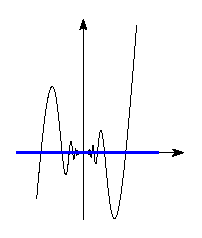
\includegraphics[width=0.2\textwidth]{21_3.eps}
	\caption{Касательная функции $f(x) = x^2 \sin{\frac{1}{x}}$ в точке $(0,0)$ пересекает график функции.}
	\label{21_3}
\end{figure}

\begin{prop}
	Касательная - это предельное положение секущей, то есть секущая: $y = \tfrac{f(b) - f(a)}{b - a}(x-a) + f(a)$. Наклон секущей $\tfrac{f(b) - f(a)}{b - a} \to f^\prime(a)$, при $b \to a$.
\end{prop}
\begin{proof}
	Очевидно из определения производной.
\end{proof}

\begin{rem}
	Когда $b \to a$, то наклон секущей стремится к наклону касательной. Приращение функции состоит из дифференциала, приближающего это приращение и погрешности этого приближения, которая ведет себя как $\alpha(h)h$. 
\end{rem}

\begin{figure}[H]
	\centering
	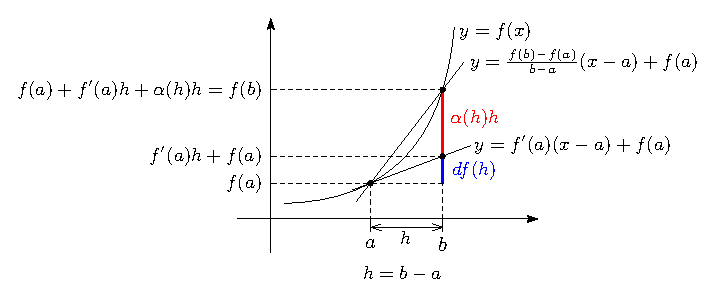
\includegraphics[width=0.75\textwidth]{21_4.eps}
	\caption{Приращение функции состоит из дифференциала и погрешности приближения.}
	\label{21_4}
\end{figure}


\end{document}